\section{Keiper Li coefficients from the P\'olya density}\label{ch:li}

The P\'olya density that computes the law of the clock also computes the coefficients of Li's criterion \cite{Li97}, which states that RH holds if and only if
\[
\lambda_n=\sum_\rho\Big[1-\Big(1-\frac1\rho\Big)^n\Big]\ge0\qquad\text{for every }n\ge1,
\]
the sum over the zeros taken in conjugate pairs. Keiper \cite{Keiper92} introduced the coefficients $\lambda_n$ and computed them before Li proved the criterion, and Bombieri and Lagarias \cite{BL99} derived an arithmetic expression for them from the explicit formula and related the criterion to Weil's.

\subsection{Taylor coefficients of \texorpdfstring{$\log\xi$}{log xi} at \texorpdfstring{$s=1$}{s=1}}\label{sec:ch20:compute}

Li \cite{Li97} expresses the coefficients as derivatives at $s=1$,
\[
\lambda_n=\frac1{(n-1)!}\frac{d^n}{ds^n}\Big[s^{n-1}\log\xi(s)\Big]_{s=1}.
\]
With $\log\xi(1+w)=\sum_{k\ge0}a_kw^k$ and $(1+w)^{n-1}=\sum_j\binom{n-1}jw^j$, comparing the coefficients of $w^n$ gives
\begin{equation}\label{eq:ch20:li}
\lambda_n=n\sum_{j=0}^{n-1}\binom{n-1}j\,a_{n-j},
\end{equation}
so the computation reduces to the Taylor coefficients of $\log\xi$ at $s=1$. The zeros nearest to $s=1$ are $\frac12\pm14.1347i$, so $\log\xi(1+w)$ is analytic in the disc $|w|<R$, where $R=|\rho_1-1|=14.1436$.

The sum \eqref{eq:ch20:li} is exact, but its terms can be larger than $\lambda_n$. The Hadamard product $\xi(1+w)=\xi(1)\prod_\rho(1-w/(\rho-1))$ gives $ma_m=-\sum_\rho(\rho-1)^{-m}$ for $m\ge2$, and for large $m$ the two zeros nearest to $s=1$ dominate this sum, so that $|ma_m|$ is at most about $2R^{-m}$. Since $n\binom{n-1}{m-1}=m\binom nm$, the terms of \eqref{eq:ch20:li} are $\binom nm\,ma_m$ with $m=n-j$, and for large $n$ their absolute sum is at most about $2(1+1/R)^n$. Cancellation therefore costs at most about $\log_{10}\big(2(1+1/R)^n/\lambda_n\big)$ digits. This grows like $n\log_{10}(1+1/R)\approx0.03n$ and is about one digit at $n=100$, where $2(1+1/R)^{100}\approx1.9\times10^3$ and $\lambda_{100}=118.6$.

We compute the $a_k$ by the trapezoid rule for the Cauchy integral on the circle $|w|=6$,
\[
a_k\approx\frac1{Nr^k}\sum_{j=0}^{N-1}\log\xi\big(1+re^{2\pi ij/N}\big)e^{-2\pi ijk/N},\qquad r=6,\ N=512,
\]
which converges geometrically. The rule returns $a_k+a_{k+N}r^N+a_{k+2N}r^{2N}+\cdots$, so aliasing changes $a_k$ by a relative amount of about $(r/R)^N\approx10^{-191}$. Rounding errors in the sum are amplified in $a_k$ by about $(R/r)^k$, which is $10^{37}$ at $k=100$ and is absorbed by the working precision.

Each value $\xi(1+w)=\xi(\frac12+(\frac12+w))$ comes from the P\'olya route at $600$ bits; the imaginary part of $\frac12+w$ never exceeds $6$, so the P\'olya sum loses almost nothing to cancellation. The principal branch of the logarithm is the analytic one, because $|\arg\xi(1+w)|<1$ on the circle: in the Hadamard product \eqref{eq:ch2:hadamard} with $s=\frac12+w$, so that $|s|\le6.5$, the factor $1+s^2/\gamma^2$ of the zeros $\frac12\pm i\gamma$ has argument at most $\arcsin(6.5^2/\gamma^2)\le1.01\cdot6.5^2/\gamma^2$, and since $\sum_{\gamma>0}\gamma^{-2}=0.0231$ these arguments add up to less than $0.99$.

The first coefficient has the closed form $\lambda_1=1+\frac{\gamma_E}2-\frac12\log4\pi$, where $\gamma_E$ is Euler's constant. The P\'olya computation gives
\[
\lambda_1=0.02309570896612103381431025,
\]
in agreement with the closed form to all twenty five digits shown. The same number $\lambda_1=\sum_\rho\rho^{-1}=(\xi'/\xi)(1)$ reappears at the basepoint one (Section~\ref{bp:sec:thorin}): the shifted clock $T_1$ there, with Laplace transform $\xi(1)/\xi(1+\sqrt u)=1-\lambda_1\sqrt u+O(u)$ near $u=0$, has a tail of order $x^{-1/2}$, and $\lambda_1/\pi$ is its Thorin density at the origin in the chart $\theta=\sqrt z$. Table~\ref{tab:ch20:li} lists further values with Keiper's asymptotic $\lambda_n\approx\frac n2(\log n-1-\log2\pi+\gamma_E)$ \cite{Keiper92}.

\begin{table}[htbp]
\centering\small
\begin{tabular}{rll}
\toprule
$n$ & $\lambda_n$ (P\'olya) & Keiper asymptotic\\
\midrule
1 & 0.023095708966121033814 & $-1.13$\\
2 & 0.092345735228046670386 & $-1.57$\\
3 & 0.20763892055432480379 & $-1.74$\\
5 & 0.57554271446117745243 & $-1.63$\\
10 & 2.2793393631931577437 & 0.21\\
20 & 8.7692768720932151296 & 7.35\\
50 & 43.531096488374019299 & 41.28\\
100 & 118.60377537679132993 & 117.23\\
\bottomrule
\end{tabular}
\caption{Keiper Li coefficients from the P\'olya density (all digits shown are correct) and Keiper's leading asymptotic, which becomes accurate only for large $n$.}
\label{tab:ch20:li}
\end{table}

\subsection{Li's criterion as positivity of the Thorin functional}\label{sec:ch20:thorin}

Li's criterion is a statement about the Thorin functional $U$ of Section~\ref{ch:arith}, which has a unit atom at $-(\rho-\frac12)^2$ for each pair $\{\rho,1-\rho\}$ of zeros, on the line or off it. For a zero $\rho$ put $q=1-1/\rho$. Then $1-1/(1-\rho)=1/q$, so the pair contributes $2-q^n-q^{-n}$ to $\lambda_n$; and if $a=-(\rho-\frac12)^2$, with the square root chosen so that $\rho-\frac12=i\sqrt a$, then $q=(2\sqrt a+i)/(2\sqrt a-i)$. This proves the following.

\begin{proposition}\label{prop:ch20:thorin}
Without any hypothesis on the zeros,
\[
\lambda_n=\sum_{\{\rho,1-\rho\}}\varphi_n\Big(-\big(\rho-\tfrac12\big)^2\Big)=\langle U,\varphi_n\rangle,
\]
where
\[
\varphi_n(z)=2-\Big(\frac{2\sqrt z+i}{2\sqrt z-i}\Big)^n-\Big(\frac{2\sqrt z-i}{2\sqrt z+i}\Big)^n
\]
is a rational function of $z$, and $\varphi_n(z)=4\sin^2\big(n\arctan\frac1{2\sqrt z}\big)\ge0$ for $z>0$.
\end{proposition}

The two fractions are exchanged when $\sqrt z$ changes sign, so $\varphi_n$ is a rational function of $z$, with a pole of order $n$ at $z=-\frac14$. At infinity $\varphi_n(z)\sim n^2/z$, so the sum converges absolutely.

For $z>0$ the two fractions are conjugate numbers of modulus one. On the critical line, for $\rho=\frac12+i\gamma$ with $\gamma>0$, the number $1-1/\rho=(\rho-1)/\rho$ has modulus one and argument $\phi_\gamma=2\arctan\frac1{2\gamma}$, and the conjugate zero gives $-\phi_\gamma$. Adding the contributions of $\rho$ and $\bar\rho$,
\[
\lambda_n=\sum_{\gamma>0}2\big(1-\cos(n\phi_\gamma)\big)=\sum_{\gamma>0}4\sin^2\Big(n\arctan\frac1{2\gamma}\Big)\qquad\text{under RH}.
\]
Li's criterion thus says that RH holds if and only if $\langle U,\varphi_n\rangle\ge0$ for every $n$, that is, the Thorin functional is nonnegative on the cone spanned by the $\varphi_n$.

The test function $\varphi_n$ is about $n^2/z$ for $\sqrt z\gg n$ and oscillates between $0$ and $4$ for $\sqrt z\lesssim n/\pi$, so $\lambda_n$ weighs the zeros below height of order $n$ at full size and the higher zeros by about $n^2/\gamma^2$ (Figure~\ref{fig:ch20:test}). Every computed $\lambda_n$ is positive, as it must be: every zero below height $3\times10^{12}$ lies on the line \cite{PT21} and contributes a nonnegative term, while a zero at height $\gamma\gg n$ contributes only about $n^2/\gamma^2$ in absolute value, so the zeros above that height cannot change the sign of $\lambda_n$ for $n\le100$.

\begin{figure}[htbp]
\centering
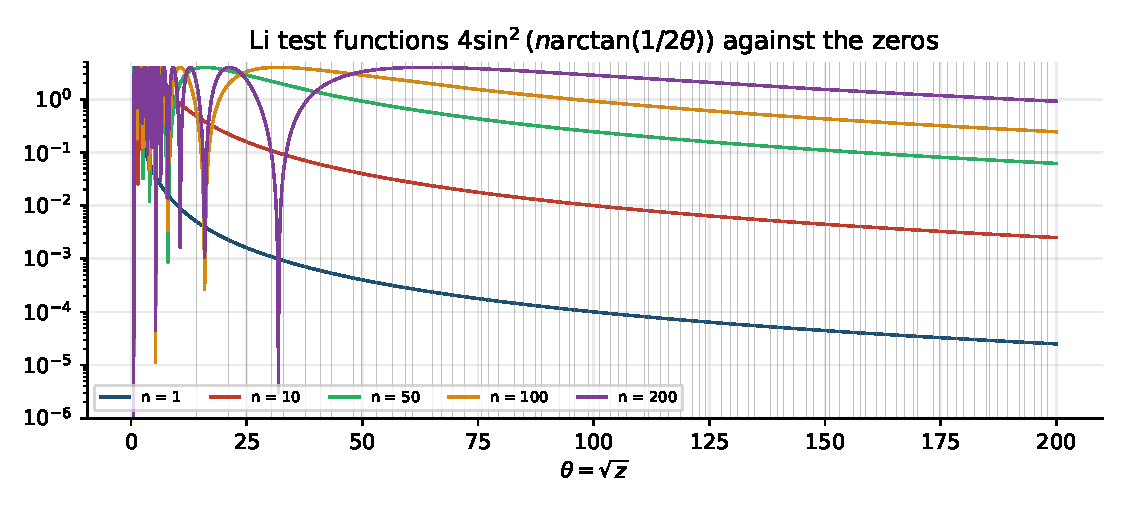
\includegraphics[width=0.9\textwidth]{fig/litest.pdf}
\caption{The Li test functions $4\sin^2(n\arctan\frac1{2\theta})$ for $n=1,10,50,100,200$, in the square root chart $\theta=\sqrt z$, against the zeros below height $200$ (grey vertical lines). Larger $n$ probes higher zeros.}
\label{fig:ch20:test}
\end{figure}

An off line zero makes $|1-1/\rho|\ne1$. For $\rho=\frac12-d+i\gamma$ with $d>0$ one has $|1-1/\rho|^2=1+2d/((\frac12-d)^2+\gamma^2)$, so for large $n$ the term $(1-1/\rho)^n$ grows like $e^{nd/\gamma^2}$, and this is how a failure of RH would eventually make $\lambda_n$ negative (Exercise~\ref{ex:ch20:offline}). Since the exponent is $nd/\gamma^2$, the index at which this happens grows with the height of the zero, so finitely many coefficients, like the finite tests of Section~\ref{ch:finite} (Table~\ref{tab:ch13:see}), cannot exclude an off line zero at great height.

Summing $4\sin^2(n\arctan\frac1{2\gamma})$ over the first $1700$ zeros, computed with \texttt{mpmath} \cite{mpmath} as in Section~\ref{ch:distances}, and adding the tail above $\gamma_{1700}$ with the smooth zero density $\log(\gamma/2\pi)/2\pi$ gives the P\'olya values with relative residuals near $5\times10^{-6}$ for $n\le20$ and $10^{-5}$ at $n=100$. The absolute residual grows like $n^2$ and comes from the cutoff: at $\gamma_{1700}$ the zero count exceeds its smooth part by about one half, so the smooth tail counts about half a term, $\frac12\varphi_n(\gamma_{1700}^2)\approx n^2/(2\gamma_{1700}^2)$, too many.

As a diagnostic the coefficients are poorly localised, so $\lambda_n$ behaves like the heat trace and Bernstein diagnostics of Table~\ref{tab:ch3:diag} and unlike the Thorin density, which is local in the ordinate.

Weil's criterion has the same form as Li's, with the functions of the class $\mathcal T$ of Section~\ref{ch:arith} that are nonnegative on $(0,\infty)$ in place of the $\varphi_n$ (Section~\ref{sec:ch10:positivity}), but the two cones are different. The pole of $\varphi_n$ lies at $-\frac14$, the point at which \eqref{eq:ch14:U} evaluates its test functions, inside the region where $\mathcal T$ requires holomorphy, and $\varphi_n$ decays only like $1/z$. So $\varphi_n$ is not in $\mathcal T$, $\langle U,\varphi_n\rangle$ is defined through the zeros, and the prime side of $\lambda_n$ is the regularised arithmetic formula of Bombieri and Lagarias \cite{BL99}.
